%%
%% This is file `sample-sigconf.tex',
%% generated with the docstrip utility.
%%
%% The original source files were:
%%
%% samples.dtx  (with options: `all,proceedings,bibtex,sigconf')
%%
%% IMPORTANT NOTICE:
%%
%% For the copyright see the source file.
%%
%% Any modified versions of this file must be renamed
%% with new filenames distinct from sample-sigconf.tex.
%%
%% For distribution of the original source see the terms
%% for copying and modification in the file samples.dtx.
%%
%% This generated file may be distributed as long as the
%% original source files, as listed above, are part of the
%% same distribution. (The sources need not necessarily be
%% in the same archive or directory.)
%%
%%
%% Commands for TeXCount
%TC:macro~\cite [option:text,text]
%TC:macro~\citep [option:text,text]
%TC:macro~\citet [option:text,text]
%TC:envir table 0 1
%TC:envir table* 0 1
%TC:envir tabular [ignore] word
%TC:envir displaymath 0 word
%TC:envir math 0 word
%TC:envir comment 0 0
%%
%% The first command in your LaTeX source must be the \documentclass
%% command.
%%
%% For submission and review of your manuscript please change the
%% command to \documentclass[manuscript, screen, review]{acmart}.

\documentclass[sigconf]{acmart}
%%
%% \BibTeX command to typeset BibTeX logo in the docs
\AtBeginDocument{%
  \providecommand\BibTeX{{%
    Bib\TeX}}}

\setcopyright{acmlicensed}
\copyrightyear{2018}
\acmYear{2018}
\acmDOI{XXXXXXX.XXXXXXX}
\acmConference[Conference acronym 'XX]{Make sure to enter the correct
  conference title from your rights confirmation emai}{June 03--05,
  2018}{Woodstock, NY}
\acmISBN{978-1-4503-XXXX-X/18/06}

\usepackage[ruled,vlined]{algorithm2e}
\SetKwInput{KwGlobalIn}{Global Mem Input}
\SetKwInput{KwSharedIn}{Shared Mem Input}
\SetKwInput{KwSharedOut}{Shared Mem Output}
\SetKwInput{KwGlobalOut}{Global Mem Output}
\SetKwInput{KwConstants}{Constants}

\usepackage{amsmath}
\usepackage{mathtools}
\usepackage{listings}
\usepackage{subcaption}
\newcommand{\thomas}[1]{{\footnotesize\color{orange}[Thomas: #1]}}
\newcommand{\john}[1]{{\footnotesize\color{cyan}[John: #1]}}
\newcommand{\raph}[1]{{\footnotesize\color{magenta}[Raph: #1]}}

\begin{document}

\title{Decoupled Fallback: A Portable Single-Pass GPU Scan}

\author{Thomas Smith}
\affiliation{%
\institution{Google}
\country{USA}}

\author{Raph Levien}
\affiliation{%
  \institution{Google}
  \country{USA}
}

\author{John D. Owens}
\affiliation{%
  \institution{University of California, Davis}
  \country{USA}}
  \additionalaffiliation{%
  \institution{Google}
  \country{USA}
}

\renewcommand{\shortauthors}{Smith et al.}

\begin{abstract}
  We present \emph{Decoupled Fallback}, a method that enables single-pass \emph{Chained-Scans} to run on hardware without \emph{Forward-Progress Guarantees} (FPG) while avoiding deadlock. Additionally, we introduce a tile state representation for \emph{Chained-Scans} that does not rely on 64-bit atomics or memory fences for correctness, along with a subgroup-size-agnostic intra-workgroup implementation. On an FPG-lacking device---Apple M1 Pro (8+2)---\emph{Decoupled-Fallback} achieves near-\emph{memcopy} speeds for inclusive prefix sum in WGPU and realizes the full theoretically expected 50\% speedup over the slower \emph{Reduce-then-Scan} approach. We further demonstrate the resilience of \emph{Decoupled-Fallback} against \emph{unfair} schedulers by emulating blocking at rates of up to 50\%, showing that it maintains superior performance over \emph{Reduce-then-Scan} even under extreme contention.
\end{abstract}

\begin{CCSXML}
  <ccs2012>
  <concept>
  <concept_id>00000000.0000000.0000000</concept_id>
  <concept_desc>Do Not Use This Code, Generate the Correct Terms for Your Paper</concept_desc>
  <concept_significance>500</concept_significance>
  </concept>
  <concept>
  <concept_id>00000000.00000000.00000000</concept_id>
  <concept_desc>Do Not Use This Code, Generate the Correct Terms for Your Paper</concept_desc>
  <concept_significance>300</concept_significance>
  </concept>
  <concept>
  <concept_id>00000000.00000000.00000000</concept_id>
  <concept_desc>Do Not Use This Code, Generate the Correct Terms for Your Paper</concept_desc>
  <concept_significance>100</concept_significance>
  </concept>
  <concept>
  <concept_id>00000000.00000000.00000000</concept_id>
  <concept_desc>Do Not Use This Code, Generate the Correct Terms for Your Paper</concept_desc>
  <concept_significance>100</concept_significance>
  </concept>
  </ccs2012>
\end{CCSXML}

\ccsdesc[500]{Do Not Use This Code~Generate the Correct Terms for Your Paper}
\ccsdesc[300]{Do Not Use This Code~Generate the Correct Terms for Your Paper}
\ccsdesc{Do Not Use This Code~Generate the Correct Terms for Your Paper}
\ccsdesc[100]{Do Not Use This Code~Generate the Correct Terms for Your Paper}

\keywords{Do, Not, Us, This, Code, Put, the, Correct, Terms, for,
  Your, Paper}

\received{20 February 2007}
\received[revised]{12 March 2009}
\received[accepted]{5 June 2009}

\maketitle

\section{Introduction (WIP)}
 (Tell readers we are targeting WebGPU)
 (Speed of light definition here)
\subsection{Goals of a Scan Implementation}
\begin{itemize}
  \item \textbf{Minimal global memory access:} the scan should minimize global memory access to the theoretical minimum of $2n$.
  \item \textbf{Fully saturates global memory bandwidth:} the scan should be capable of fully saturating the global memory bandwidth.
  \item \textbf{Portability:} the scan should be portable across hardware vendors and architectures.
\end{itemize}
Our method retains the best aspects of the \emph{Chained-Scan} architecture, while eliminating the need for forward progress guarantees. It is designed to operate on arbitrary hardware, support arbitrary monoids, process inputs of arbitrary size, and support arbitrary 32-bit and 64-bit data types.
\subsection{Goals}
This work is guided by two main goals:
\begin{enumerate}
  \item \textbf{Portability}: we want to develop a scan implementation that retains the benefits of the \emph{Chained-Scan} architecture but is also suitable for a diverse range of hardware vendors and architectures, including those without FPG or support for 64-bit atomics.
  \item \textbf{Performance}: we aim for near speed-of-light execution to the greatest extent possible allowed by the underlying hardware and programming model.
\end{enumerate}

\noindent
To ground these objectives, we select the WebGPU shading language (WGSL) and the WebGPU standard as our target environment. WGSL is a meta-level shading language which is translated and compiled as necessary for backend graphics APIs---D3D12, Vulkan, and Metal---and as such, WGSL implementations are bound by the minimum capability across all backends. Because WGSL must operate within this limited capability space, it inherently embodies the challenge of portability.

\subsection{Non Goals}
Although our goal is to create a fully portable and highly performant scan implementation, we are constrained by underlying hardware platforms and programming models. As discussed in more detail in \emph{Limits on the Speed-of-Light}, not all architectures offer atomic operations that are sufficiently fast enough or scheduling models that are sufficiently fair enough to attain speed-of-light performance, and thus we cannot guarantee such performance. Although we are cognizant of the risks posed by subgroup divergence, subgroup functions in shading languages do not allow explicit divergence control,\footnote{For example, CUDA allows developers to explicitly provision subgroup functions with a mask of the threads that will participate in them.} placing a solution to subgroup divergence issues outside our scope. Lastly, we do not investigate alternative $O(2n)$ scan architectures beyond \emph{Chained-Scan}.

\subsection{Contributions}
\begin{enumerate}
  \item Decoupled-Fallback
  \item Split-Method
  \item Subgroup-Size Agnostic stuff
\end{enumerate}

\section{Background}
\subsection{Virtualization and Scheduling in the GPU programming model}
Contemporary GPUs are hierarchically organized, massively parallel processors designed to prioritize throughput over latency. (one sentence on thread hierarchy maybe). As comprehensive descriptions of the GPU programming model~\cite{} already exist, we focus on the aspects most relevant to this work: scheduling and synchronization.

On GPU hardware, scheduling is divided into two levels: a \emph{workgroup} scheduler, which manages kernel launches and maps virtual processors, workgroups, to physical processors, \emph{multiprocessors}, and a \emph{subgroup} scheduler, responsible for selecting which of the currently \emph{occupant} subgroups on a multiprocessor for execution. The GPU programming model virtualizes processors to ensure GPU programs---\emph{kernels}---remain portable across hardware with differing physical resources. Effective virtualization requires \emph{oversubscription}, a programming paradigm where tasks are (over)partitioned in such a way that kernels request more virtual processors than are physically available. As a result, a single multiprocessor may host multiple workgroups simultaneously. However, as a consequence of virtualization, the developer relinquishes control over the order in which workgroups are launched, and once a workgroup begins execution on a multiprocessor, it must run to completion and cannot context switch.

\subsubsection{Inter-Workgroup Barriers}
The virtualization of processors introduces an emergent high-level limitation: the absence of an inter-workgroup barrier. As previously mentioned, workgroups cannot context switch. Although contemporary GPU hardware~\cite{} supports workgroup preemption for prioritizing real-time tasks or managing multi-process workloads, this functionality is deliberately excluded from the GPU programming model. This stems from the prohibitively high overhead in latency and storage associated with moving workgroup contexts on and off chip. In the oversubscription paradigm, where the number of workgroups is theoretically unbound and typically far exceeds the available multiprocessors, every invocation of such a barrier would necessitate context-switching between all launched workgroups. Due to this high cost, no GPU programming environment furnishes developers with a true unbounded-launch inter-workgroup barrier.\footnote{CUDA recently introduced \emph{Thread Block Cluster} synchronization~\cite{NvidiaCudaGuide}, but it is almost certainly designed to operate within the \emph{Persistent-Thread}~\cite{gupta2012} paradigm, rather than serving as a barrier across an unbounded launch.} Instead, when inter-workgroup synchronization is necessary, developers must rely on kernel launches as synchronization points. However, kernel launches are suboptimal as barriers: they incur overheads due to the heterogeneous nature of the operation, and all execution context is lost between launches.

\subsubsection{Fairness and Progress}
Because multiple workgroups may reside on a single multiprocessor, two key issues arise at the subgroup scheduling level: \emph{fairness}---how evenly execution resources are distributed among subgroups---and \emph{progress guarantees}---ensuring that subgroups eventually make progress towards termination. However, the term "fairness" is used differently across the literature, leading to potential confusion. Sorensen et al.~\cite{sorensen2016,sorensen2018,sorensen2021}, whose work provides the most comprehensive taxonomy of progress models to date, use "fairness" specifically to describe differing levels of progress guarantees. In contrast, NVIDIA publications~\cite{4523358,Merrill2016} define "fairness" in terms of the distribution of execution resources among subgroups. In this work, we adopt NVIDIA's terminology.

\thomas{A scheduler may be fair but may not have FPG (M1 Pro for example); a scheduler may have FPG but may not be fair (ARM Mali). \newline
  Sorensen calls FPG "fairness:" "We have described two schedulers: fair and unfair, under which starvation-freedom for blocking idioms is either always or never guaranteed."\newline
  NVIDIA, by contrast uses fairness in line with our language. From Tesla architecture: \newline
  "A scoreboard qualifies each warp for issue each cycle. The instruction scheduler prioritizes all ready warps and selects the one with highest priority for issue. Prioritization considers warp type, instruction type, and 'fairness' to all warps executing in the SM\@." \newline
  From DecoupledLookback: \newline
  "Safety. The algorithm will run to completion if the system guarantees forward-progress for all processors." \newline
  "Blocking will be minimal for systems that provide fair or nearly-fair scheduling. Fairness ensures that all processors will have recorded their aggregates in roughly the same amount of time."
}

\subsection{The Scan Primitive}\label{sec:the-scan-primitive}
The study of \emph{scan} (\emph{parallel prefix}) networks traces back to the design of carry-lookahead adder circuits and beyond~\cite{5219801,10.5555/1098666}. A scan is typically defined on a monoid \( M \), characterized by a binary reduction operator \( \oplus \) and an identity element \( \varepsilon \). The binary operator \( \oplus \) satisfies the closure property \( \forall a, b \in M, \ (a \oplus b) \in M \) and has an identity element \( \exists \varepsilon \in M, \ \forall a \in M, \ \varepsilon \oplus a = a \). To allow parallelization, \( \oplus \) must be associative, but it is not necessarily commutative, as demonstrated in structures like the \emph{bicyclic semigroup}~\cite{}\footnote{Despite its name, this is a monoid.} and Rabin-Karp's \emph{second fingerprinting method for string matching}~\cite[Section 6]{Karp:1987:ERP}. In a scan, the result at the \( n \)-th element is the reduction of the preceding subset of elements in the sequence. If the subset includes the \( n \)-th element, it is called \emph{inclusive}; if it excludes the \( n \)-th element, it is called \emph{exclusive}. The most common scan type is the prefix sum, where \( \oplus \) is addition. For example:
\[
  x = [x_1, x_2, x_3, \dots, x_n] \ \ \ \ \ \ \ y = [1, 1, 1, 1, 1]
\]
\[
  \text{InclusiveScan}(x, \oplus) = [x_1, x_1 \oplus x_2, x_1 \oplus x_2 \oplus x_3, \dots, x_1 \oplus x_2 \oplus \cdots \oplus x_n]
\]
\[
  \text{InclusiveScan}(y, +) = [1, 2, 3, 4, 5]
\]
Due to its significance in circuits and as a fundamental algorithmic primitive, scan has been extensively studied in both electrical engineering and computer science. Harris~\cite{1292373} offers a taxonomy that relates depth, fanout, and wire tracks, while Hinze~\cite{10.1007/978-3-540-27764-4_11} develops an algebraic framework for scans. Snir~\cite{10.1016/0196-67748690003-9} proved that depth $d$ and size $s$ are related by $s + d \ge 2n - 2$, and Fich~\cite{10.1145/800061.808738} proved that among minimum depth scans Ladner-Fischer~\cite{10.1145/322217.322232} networks have optimal size. Blelloch~\cite{Blelloch:1989:SAP} adapted scan to the PRAM model and popularized its use as an algorithmic primitive. Finally, Merrill and Garland~\cite{Merrill2016} provide a review of GPU scan implementations, complementing earlier work by Merrill and Grimshaw~\cite{Merrill2009}.

\subsection{Evolution of Inter-Workgroup Scan Architectures}
Contemporary GPU scans depart from early PRAM-like scans~\cite{} by leveraging the GPU memory hierarchy, which consists of progressively faster but increasingly private tiers. Efficient scans integrate fine-grained intra-workgroup (\emph{local}) strategies in shared memory and registers with coarse-grained inter-workgroup (\emph{global}) strategies in global memory. Given their low arithmetic intensity, local scans are inherently memory-bound, as demonstrated by Merrill and Grimshaw~\cite{}. Consequently, recent scan optimizations have shifted toward refining global strategies, particularly inter-workgroup coordination and synchronization. This section reviews three key approaches---\emph{Scan-then-Propagate}, \emph{Reduce-then-Scan}, and \emph{Chained-Scan}---analyzing their handling of inter-workgroup dependencies and efficiency in minimizing global memory access while maximizing bandwidth utilization. \thomas{I have written this paragraph like twenty times now, and it's still odious.}

\subsubsection{Scan-then-Propagate}
Introduced by Sengupta et al.~\cite{10.5555/1280094.1280110}, the \emph{Scan-then-Propagate}~\cite{GPUGems3, Sengupta2011} extends intra-workgroup scans to large inputs by resolving inter-workgroup dependencies in three phases:
\begin{enumerate}
  \item \textbf{Intra-Workgroup (Local) Scan:}  Each workgroup performs an inclusive scan on its assigned work tile, storing local results and reductions in global memory.
  \item \textbf{Spine Scan:} The workgroup reductions, collectively forming the \emph{spine}, are gathered and scanned to compute the \emph{root}, resolving dependencies between work tiles. For large scans, this stage is an insignificant amount of work compared to the first and third.
  \item \textbf{Propagation:} Each workgroup retrieves its portion of the root and adds it to the local scan output.
\end{enumerate}

The absence of inter-workgroup barriers necessitates separate kernel launches for dependency resolution, inherently structuring \emph{Scan-then-Propagate} into three phases. Sengupta et al.'s implementation further complicates this by using recursion to handle arbitrarily large inputs. As the size of a work tile limits the maximum number of elements processed without inter-workgroup dependency resolution, the three-phase structure must be recursively applied until the spine size fits within a single work tile. Thus, an input of size $n$ and a work tile of size $t$ results in a recursive depth of $\lceil \log_t n \rceil$, and $2\cdot\lceil \log_t n \rceil - 1$ kernel launches. Each recursive step $k$ processes $n/t^k$ tiles, leading to a total of $\sum_{k=1}^{\lceil \log_t n \rceil} n/t^k \approx (n - 1)/(t - 1)$ work tiles over all steps. Since each tile moves $4t$ data ($2t$ local scan, $2t$ propagation), the total global data movement is $O\left(\frac{4t(n - 1)}{t - 1}\right) = O(4n)$.

\subsubsection{Reduce-then-Scan}
If memory bandwidth resources are sufficiently scarce relative to compute, memory-bound algorithms like scan can profit by trading additional computation for reduced memory traffic. This trade-off led to a refinement of the \emph{Scan-Then-Propagate} strategy called \emph{Reduce-Then-Scan}~\cite{10.1145/1375527.1375559, Merrill2009, 10.1109/TPDS.2012.336, 10.5555/2031978.2032029}: by storing only the work tile reduction in global memory during the first phase and performing a redundant scan in the third, it eliminates $n$ global data movement while preserving the three-phase structure:
\begin{enumerate}
  \item \textbf{Work Tile Reduction:} Each workgroup performs a pure reduction on its work tile partition, posting the result to global memory.
  \item \textbf{Spine Scan:} The spine is scanned to produce the root.
  \item \textbf{Intra-Workgroup Scan and Propagation:} Each workgroup performs the local scan on the work tile, incorporating its portion of the root as it writes to global memory.
\end{enumerate}

Merrill and Grimshaw~\cite{Merrill2009} introduced \emph{workgroup raking} to further reduce recursion overhead when the recursion depth exceeds two. Instead of recursively reducing the spine, the input is partitioned into $o$ groups, where $o$ is the total workgroup occupancy. Each workgroup sequentially processes its assigned partition, reducing the spine size to a constant and guaranteeing a recursion depth of at most two. This reduces global memory movement for the spine scan from $O(n/t)$ to $O(2o)$ and limits kernel launches to three, reducing total global memory movement to $O(3n + 4o) = O(3n)$.

Breitbart~\cite{10.5555/2031978.2032029} applied Gupta et al.'s \emph{Persistent-Threads}~\cite{gupta2012} to scan, eliminating kernel launch overheads. Recognizing that raking naturally aligns with this paradigm, Breitbart replaced kernel launches with an atomics-based inter-workgroup barrier. Since multiprocessors are not oversubscribed in raking, workgroups persist for the entire kernel duration, allowing synchronization at the barrier without context switching. Despite maintaining $O(3n)$ global memory movement, consolidating the scan into a single kernel minimizes launch overheads.

\subsubsection{Chained-Scan, Stream-Scan}
First introduced by Yan et al.~\cite{10.1145/2442516.2442539} in \emph{Stream-Scan}, the key innovation of the \emph{Chained-Scan} architecture lies in its hybridization of parallel and serial strategies: achieving parallelism at the intra-workgroup level while minimizing global data movement through serial scan operations at the inter-workgroup level. Instead of using kernel launches as inter-workgroup synchronization points, \emph{Chained-Scans} launch a single kernel that assigns work tiles in a serial order to workgroups, utilizing atomics and bit-packed status flags to ensure coherent views of data. To enforce this serial ordering, work tiles are dynamically assigned using atomic increment operations, rather than arbitrary assignment based on virtualized workgroup indices. This shifts dependency resolution from explicit synchronization via barrier-like structures to implicit synchronization via access order. As a result, each element is read and written exactly once, achieving the theoretical minimum of $2n$.

In any \emph{Chained-Scan}, once a workgroup computes its local scan, it must complete two objectives: communicate its reduction to successor tiles and resolve dependencies by incorporating the reductions of all preceding tiles. This process, which we refer to as \emph{Chained Propagation}, defines the set of inter-workgroup techniques that facilitate dependency resolution. In \emph{StreamScan}, these two objectives are combined into a single phase, where each workgroup waits for its immediate predecessor to complete, ingests the predecessor's reduction, and posts the resulting \emph{inclusive} reduction for its immediate successor to consume. During this waiting period, the workgroup is continually scheduled, and the \emph{progress} of other workgroups must be guaranteed to prevent the spinning workgroup from starving its dependent predecessors of execution, which could result in deadlock.

While \emph{StreamScan} successfully reduces per-element device memory accesses to two, it does not consistently saturate global memory bandwidth, preventing it from achieving speed-of-light performance. This limitation arises because a workgroup in \emph{StreamScan} cannot post its reduction to global memory until it has received the result of its immediate predecessor. While this results in efficient $O(n/t)$ communication of reductions, and $O(2n+ n/t)= O(2n)$ total data movement, the sequential dependency creates a bottleneck that limits performance to the rate at which reductions propagate through device memory. Although this can be mitigated by increasing the size of the work tile, limited on-chip resources preclude scaling the tile size indefinitely. Moreover, this approach is unsuitable for a portable environment, as excessively large work tiles risk reducing occupancy on less capable hardware.

\subsubsection{Chained-Scan, Decoupled-Lookback}
Introduced by Merrill and Garland, the \emph{Decoupled-Lookback} technique refines \emph{Chained Propagation} by separating reduction communication from dependency resolution, mitigating bottlenecks caused by propagation latency. In this approach, each workgroup posts its local reduction to global memory and then performs a \emph{lookback}---a serial traversal backward along the spine---to compute its inclusive reduction. Work and memory accesses are constant-bounded to the workgroup occupancy $o$ by posting the inclusive reduction after the lookback. However, granting each workgroup control over its dependency resolution does not eliminate reliance on \emph{progress guarantees}, as workgroups must still spin on tiles that have yet to post their reductions, risking deadlock.

Although \emph{Decoupled-Lookback} increases global memory access during the propagation phase to $O(o(n/t))$, the serial ordering of work tile processing confines spine memory accesses to a roughly $o$-width sliding window, making them highly likely to be cache-resident. As a result, the additional global memory traffic along the spine introduces a negligible latency overhead. With total global memory movement of $O(2n+o(n/t))= O(2n)$, \emph{Decoupled-Lookback} achieves full utilization of device memory bandwidth and delivers speed-of-light performance without the work tile size tuning required by \emph{Stream-Scan}.

\subsection{Ideal Scan Architecture}
Beyond their differences in speed, \emph{Chained-Scan} and \emph{Reduce-Then-Scan} embody two fundamentally contrasting paradigms. By eliding explicit inter-workgroup synchronization, \emph{Chained-Scan} aligns naturally with the oversubscription paradigm, delegating occupancy management to the hardware scheduler. In contrast, the raking approach inherent to \emph{Reduce-Then-Scan} mandates the fixed-launch paradigm, necessitating explicit control over occupancy and potentially synchronization.

Fixed-launch approaches demand substantial developer effort, requiring either tuning of workgroup launch sizes across target devices or occupancy discovery. Moreover, previous workgroup occupancy discovery techniques, such as the one proposed by Sorensen et al.~\cite{sorensen2016}, are infeasible to implement in WebGPU due to their reliance on memory fences---a feature not supported by the specification.\footnote{Our implementation includes a fenceless occupancy discovery method amenable to the WebGPU environment, but its description is beyond the scope of this work.}

Hardware-level considerations further underscore the limitations of fixed-launches. On GPUs where the global memory data cache is indexed by physical addresses---and therefore requires lookups in \emph{translation lookaside buffers} (TLBs)---fixed-launches can lead to performance degradation due to cache thrashing. This issue occurs when task sizes are large enough that each workgroup accesses its own unique page entry, and the device lacks sufficient TLB coverage to support the memory access patterns of all workgroups. Although this behavior typically does not manifest with simple monoids, more complex monoids with \emph{struct-of-array} memory access patterns---or applications like radix sorting, where the scattering phase of each pass results in $radixDigits \cdot o$ unique memory locations---may experience significant performance degradation.

Thus, oversubscription and \emph{Chained-Scan} emerges as the preferred architecture, as it naturally aligns with portability by leveraging hardware schedulers to dynamically manage occupancy across diverse architectures without requiring developer intervention. Furthermore, as a single kernel with inherently serial ordering, \emph{Chained-Scan} is suitable for \emph{in-situ} operations, augmenting practical routines such as data deduplication, sparse data compaction, error correction, and interval merging.

But, while \emph{Chained-Scan} with \emph{Decoupled Lookback} appears to be the ideal scan architecture in terms of its theoretical and implementation characteristics, it falls short in fully meeting the criterion of \emph{portability}. This limitation arises because \emph{Chained-Scan} depends on a \emph{forward-progress guarantee}, a feature provided by NVIDIA devices but notably lacking on Apple's M-series and ARM GPUs~\cite{sorensen2021}. Without this guarantee, \emph{Chained-Scan} is highly prone to catastrophic failure in the form of deadlocking.

\subsection{Why does \emph{Chained-Scan} Rely on Forward-Progress Guarantees?}
A \emph{forward-progress guarantee} (FPG) ensures that all occupant subgroups (from possibly different workgroups) eventually make progress toward termination, preventing indefinite starvation. Sorensen et al.~\cite{sorensen2018,sorensen2021} provide the most comprehensive analysis of GPU schedulers, classifying \emph{Chained-Scan} as FPG-reliant. However, their work primarily focuses on formalizing progress models rather than their direct application to specific algorithms.
\thomas{Sorensen places Chained-Scan into the HSA category, but it is unclear if this is correct. The definition of HSA is \newline ``Threads for which fair execution is guaranteed: The thread with the lowest id that has not yet terminated'' \newline However, as Chained-Scan and other serially ordered algorithms no longer use the virtual ID provided by the workgroup scheduler, is fair execution still guaranteed under HSA? It seems that it should be classified under OBE\@.} \john{I don't have an opinion on this, you're familiar with this and I'm not, but this seems like a good footnote. Or we can ask Tyler.}

The challenges faced by \emph{Chained-Scan} resemble the \emph{Dining Philosophers Problem}, where competing tasks share limited resources, risking deadlock. Coffman et al.~\cite{10.1145/356586.356588} define four conditions necessary for deadlock:
\begin{enumerate}
  \item \textbf{Mutual Exclusion}: Tasks claim exclusive control of resources they require.
  \item \textbf{Resource Holding}: Tasks hold acquired resources while waiting.
  \item \textbf{No Preemption}: A resource cannot be removed from a task before completion.
  \item \textbf{Circular Dependency}:
        \begin{enumerate}
          \item Dependency Relationships: A dependency exists such that each task holds one or more resources that are required by proceeding tasks.
          \item Circular Ordering: A circular chain of tasks exists.
        \end{enumerate}
\end{enumerate}
Applying this schema to \emph{Chained-Scan}, workgroups correspond to "tasks" and work-tile reductions to "resources." Conditions 1–3 hold due to the one-to-one mapping of work tiles to workgroups and the constraints of the GPU programming model. Condition 4a is satisfied by the inter-tile dependencies, leaving condition 4b---\emph{circular ordering}---as the key concern.

Although the serial assignment of work tiles ensures that predecessor tiles are scheduled or completed, it does not guarantee their reductions will be available when a workgroup begins \emph{Chained Propagation}. This uncertainty arises because workgroups are scheduled \emph{individually}, meaning a predecessor may not have had the opportunity to compute and post its reduction. In such cases, the dependent workgroup spins, consuming execution resources while waiting. Because workgroups may share execution resources by being co-resident on the same multiprocessor\john{Question, and maybe this is worth a footnote. What if we guaranteed that no multiprocessor ever had more than one workgroup scheduled to it, say by always allocating the maximum amount of workgroup memory? Of course there would be performance issues. But does that solve the problem? Or do we descend into an analogous issue with subgroup scheduling?}, without FPG, the scheduler may indefinitely prioritize the spinning workgroup over its predecessor, preventing progress and creating a circular dependency, satisfying condition 4b and resulting in deadlock.

For example, consider a scan operation requiring two workgroups on a GPU with a single multiprocessor. Both workgroups are co-resident, but the multiprocessor has only one scheduling unit, which lacks FPG\@. Both workgroups launch and acquire their respective work tiles. The workgroup responsible for \emph{Work Tile 1} finishes first and begins spinning, repeatedly querying the memory address for the reduction of \emph{Work Tile 0}. However, because the scheduler lacks FPG, it continues scheduling \emph{Work Tile 1}, leaving \emph{Work Tile 0} starved and unable to complete its reduction. As a result, \emph{Work Tile 1} spins indefinitely, eventually triggering \emph{timeout detection and recovery} (TDR) and crashing the host program.

\subsection{Why is reliance on Forward Progress Guarantees a Portability Problem?}
The absence of FPG in key hardware segments poses a critical challenge for developers. Our testing shows that, at best, running \emph{Chained-Scan} without FPG results in severe performance degradation, and at worst, risks TDR and program crashes.
\begin{figure}
  \centering
  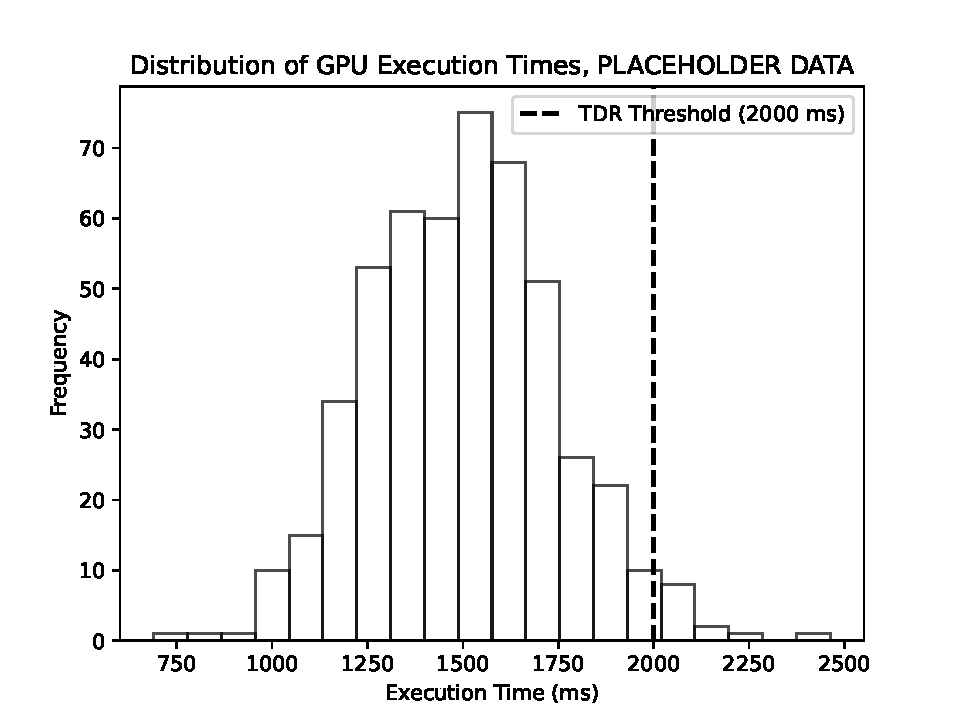
\includegraphics[width=\linewidth]{graphics/Figure_1.pdf}
  \caption{Execution times of \emph{Decoupled-Lookback (PLACEHOLDER DATA)}}
\end{figure}
Exacerbating this issue, no major graphics API provides a mechanism to query FPG support. This lack of transparency forces developers to design algorithms without knowing whether critical guarantees are available on the target hardware. In shader environments, where cross-platform portability is essential, this uncertainty compels a fallback to older, less efficient strategies like \emph{Reduce-Then-Scan}, sacrificing performance for broader compatibility.

\subsection{Earlier Attempts at Portability}
\john{I'd like Raph to chime in here. What I worry about in the way this subsection is presented is that a reviewer will say ``Oh, the fallback technique was already invented in 2021, all this paper does is makes it a little better''. On one hand I totally want Raph to get credit for this cool idea. On the other hand, writing this subsection in this way, as a citable previous publication, significantly reduces the size of the advance that this paper we're writing hopes to capture. If I'm being selfish and trying to make this paper look as good as possible, I downplay the previous work a little and don't present it as if it was a previous peer-reviewed publication. At the least I want to use the words ``blog post'' in the text here.}
Levien and Naur~\cite{Raph2021} made the first attempt at implementing a \emph{Decoupled-Lookback} approach without FPG requirements in \emph{Scalar Fallback}. Each time a workgroup spins on a preceding tile, it advances a \emph{fallback} operation by incrementally consuming the blocking tile---one element at a time. This eliminates the \emph{mutual exclusion} condition necessary for deadlock, as workgroups can operate on data from other tiles. While this may introduce redundant work when a tile is late rather than truly blocking, it guarantees termination by allowing any workgroup to complete a blocking tile’s reduction, breaking inter-workgroup dependencies.

\emph{Scalar Fallback} suffers from two primary inefficiencies. First, the fallback reduction is performed serially by a single thread, progressing only when the workgroup enters a waiting spin. This results in a $t$-sized blocking tile requiring $t$ spins to complete. Additionally, since only one thread loads elements, the associated cache line is severely underutilized. Second, once the fallback completes, the workgroup does not post its result to device memory, forcing every blocked workgroup to redundantly recompute the fallback. \john{If we can, we would like to [politely] say that this previous work was missing a key insight, e.g., while fallback can address the portability problem, \ldots\ Would we say that it's not decoupled in the way that the technique we present in this paper is? Or is the only deficiency the choice of a serial fallback?} While \emph{Scalar Fallback} achieved speed-of-light performance on hardware with FPG and executed correctly without it, its performance on the latter was inferior to \emph{Reduce then Scan}.

\section{Decoupled Fallback}
\emph{Decoupled Fallback} separates fallback operations from the lookback process, enhancing the \emph{Scalar-Fallback} technique with significantly improved fallback performance. As an extension of the \emph{Chained-Scan} architecture, it retains the advantages of high speed and oversubscription, aligning with our design requirements.

Like \emph{Scalar-Fallback}, we choose \emph{mutual exclusion} as our approach to preclude deadlocks. \emph{Dependency relationships} and \emph{no preemption} are immutable characteristics of scan and the GPU programming model, eliminating them as viable avenues for breaking deadlocking. While it may be possible to break \emph{circular ordering} by designing tile sizes such that workgroups are mapped one-to-one to multiprocessors, doing so portably is infeasible. Moreover, vendor guidance on progress guarantees among multiprocessors is also lacking, shifting rather than eliminating deadlock risks. Removing \emph{resource holding}---allowing workgroups to discard \emph{blocked} work tiles---is theoretically possible but strictly inferior to removing \emph{mutual exclusion}, as it incurs $t$ extra memory operations (discard-read-read instead of read).
\begin{algorithm}
  \small
  \SetAlgoLined
  \KwGlobalIn{%
    $\textit{in}[]$,
    $\textit{out}[]$,
    $\textit{spine}[]$,
    $\textit{tileBump}$,
  }
  \KwSharedIn{%
    $\textit{wg\_partials}[]$,
    $\textit{wg\_fallback}[]$,
    $\textit{wg\_prev\_reduction}$,
    $\textit{wg\_broadcast}$,
    $\textit{wg\_control}$,
  }
  \KwGlobalOut{$\textit{out}[]$ inclusive scan of $\textit{in}[]$}
  \KwConstants{Vectors per thread $\textit{p}$}

  \If{$\textit{threadid} = 0$}{
    $\textit{wg\_broadcast} \gets \textnormal{atomicAdd}(\&\textit{tileBump}, 1)$\;
    $\textit{wg\_control} \gets \textnormal{LOCKED}$\;
  }
  \textbf{barrier()}\;

  $\textit{part\_id} \gets \textit{wg\_broadcast}$\;

  \textit{local\_vectors}: $\textnormal{array}\langle \textnormal{vec4}\langle u32\rangle, \textit{p} \rangle$\;

  \textbf{Load}($\textit{in}$, $\textit{part\_id}$, \textit{local\_vectors})\;
  \textbf{SubgroupRake}(\textit{local\_vectors})\;

  \If{$\textnormal{highestRankLane}(\textit{threadid})$}{
    $\textit{wg\_partials}[\textit{subgroup\_id}] \gets \textit{local\_vectors}[\textit{p} - 1]$\;
  }
  \textbf{barrier()}\;

  \textbf{WorkgroupWideScan}($\textit{wg\_partials}$)\;
  \textbf{barrier()}\;

  \tcp{Chained Propagation, Decoupled Fallback}
  \While{$\textit{wg\_control} = \textnormal{LOCKED}$}{
    \textbf{Lookback}($\textit{spine}$, $\textit{wg\_prev\_reduction}$, $\textit{wg\_control}$)\;
    \textbf{barrier()}\;

    \If{$\textit{wg\_control} = \textnormal{LOCKED}$}{
      \textbf{FallbackReduce}($\textit{in}$, $\textit{wg\_fallback}$)\;
      \textbf{FallbackInsertionAttempt}($\textit{spine}$, $\textit{wg\_fallback}$, $\textit{wg\_prev\_reduction}$, $\textit{wg\_control}$)\;
      \textbf{barrier()}\;
    }
  }

  \textbf{Write}($\textit{out}$, $\textit{part\_id}$, \textit{local\_vectors}, $\textit{wg\_partials}$, $\textit{wg\_prev\_reduction}$)\;

  \caption{High-Level Scan Kernel}
\end{algorithm}

To optimize the fallback operation, we employ three strategies. Although \emph{Chained-Propagation} is performed by a single thread or subgroup, for performance reasons we want the entire workgroup to participate in the fallback. (1) First, a shared memory \emph{control flag} enables threads performing the lookback to signal the entire workgroup when a fallback is necessary. (2) Next, we limit the number of spins a thread can perform while waiting on a tile; exceeding this threshold triggers a fallback. While this approach risks redundant fallbacks---since a late tile is indistinguishable from a genuinely blocking one---exposing the maximum spin count as a tunable parameter helps minimize false positives. \john{I can see it is sensible to have a maximum spin count but I do not see how the action of exposing the maximum spin count to the programmer minimizes false positives.} (3) Finally, after completing a fallback, the workgroup attempts to post the reduction result of the blocking tile, preventing redundant fallbacks by subsequent workgroups.

The viability of \emph{Decoupled-Fallback} relies on the same cache locality properties as \emph{Decoupled-Lookback}. Since no subgroup scheduler is perfectly fair, all hardware inherently has a natural fallback rate $f$\!, independent of FPG, due to \emph{false-positive} fallback operations. As a result, memory bandwidth usage increases (and throughput decreases) from $O(fn)$ to $O((2 + f)n)$. However, as serial ordering confines spine memory accesses within an $o$-width sliding window, scan input accesses are likewise constrained to an $ot$-width window, increasing their likelihood of residing in cache. As we later empirically demonstrate, this cache residency significantly reduces memory access costs, making fallback operations predominantly compute-bound when reducing a blocking tile. Since pure reduction has minimal overhead, throughput approaches $O(2n)$ on most devices.

\section{Implementation}
At a high level, our algorithm follows a five-phase construction:
\begin{enumerate}
  \item[(0)] \textbf {Initialization}: The first thread in the workgroup atomically acquires its work-tile by atomically incrementing a value in global memory.
  \item \textbf{Load Phase}: Each thread loads $p$ vectors, consuming the input in a subgroup-blocked ordering. For a subgroup size $s$ and vector size $v$, each subgroup processes a contiguous block of size $s \cdot p \cdot v$.
  \item \textbf{Subgroup-Rake}: Each thread scans its vectors privately, then joins $p$ raking subgroup scans,
  allowing the subgroup-block scan to remain barrier-free and in registers. The subgroup-block reduction is then posted to shared memory. For a workgroup of size $w$, subgroup-raking reduces the size of the local spine to $w/s$.
  \item \textbf{Workgroup-Wide Scan}: The workgroup collectively performs a scan across the subgroup partial reductions, writing the results back to shared memory upon completion.
  \item \textbf{Chained Propagation, Decoupled Fallback}: The first subgroup in the workgroup performs a lookback operation to acquire the reduction result of all previous workgroups, engaging in fallback operations as necessary. Once completed, this subgroup posts the results to shared memory for the workgroup to consume.
  \item \textbf{Write Phase}: Each subgroup incorporates the results from the workgroup-wide scan and lookback operation to produce and write out the correct output.
\end{enumerate}
Phase 0 ensures that the work tiles are consumed in serial order. Phases 1, 2, 3, and 5 comprise the intra-workgroup scan, following a \emph{Scan-then-Propagate} strategy. Phase 4, \emph{Decoupled-Fallback}, is responsible for managing all inter-workgroup dependencies. As our loading and writing phase are typical of scan kernels, we focus here on our portability-specific adaptations.

\begin{algorithm}
  \small
  \SetAlgoLined
  \KwSharedIn{ Array of subgroup partial reductions $\textit{x}$ }
  \KwSharedOut{ Inclusive-scanned $\textit{x}$ }
  \KwConstants{ Workgroup Size $\textit{W}$, Subgroup Size $\textit{S}$ }

  $\textit{spine\_length} \gets \textit{W} / \textit{S}$\;
  $\textit{alignment} \gets 1 << \text{divRoundUp}(\log_2(\textit{spine\_length}), \log_2(\textit{S})) \cdot \log_2(\textit{S})$\;

  $\textit{stride} \gets 1$\;
  $\textit{top\_offset} \gets 0$\;

  \ForEach{$\textit{thread\_id}$ \textbf{in} $\textit{W}$ \textbf{in parallel}}{
    \For{$\textit{j} \gets \textit{S}$ \KwTo $\textit{alignment}$ \textbf{with} $\textit{j} \gets \textit{j} \cdot \textit{S}$}{
      \tcp{Brent-Kung Upsweep}

      $\textit{step} \gets \textit{spine\_length} / \textit{stride}$\;

      \If{$\textit{thread\_id} < \textit{step}$}{
        $\textit{temp} \gets \text{subgroupInclusiveScan}(\textit{x}[\textit{thread\_id} + \textit{top\_offset}])$\;
        $\textit{x}[\textit{thread\_id} + \textit{top\_offset}] \gets \textit{temp}$\;
        \If{$\text{\normalfont highestRankLane}(\textit{thread\_id})$}{
          $\textit{x}[(\textit{thread\_id} / \textit{S}) + \textit{step} + \textit{top\_offset}] \gets \textit{temp}$\;
        }
      }

      \textbf{barrier()}\;

      \tcp{Fanout}

      \If{$\textit{j} \neq \textit{S}$}{
        $\textit{reduced\_stride} \gets \textit{j} / \textit{stride}$\;
        $\textit{fanout\_index} \gets \textit{thread\_id} + \textit{reduced\_stride}$\;

        $\textit{cond1} \gets \textit{fanout\_index} < \textit{spine\_length}$\;
        $\textit{cond2} \gets (\textit{fanout\_index} \& (\textit{j} - 1)) \geq \textit{reduced\_stride}$\;

        \If{$\textit{cond1} \textbf{ \&\& } \textit{cond2}$}{
          $\textit{x}[\textit{fanout\_index}] \gets \textit{x}[\textit{fanout\_index}] + \textit{x}[((\textit{fanout\_index} / \textit{stride}) + \textit{top\_offset}) - 1]$\;
        }
      }
      $\textit{stride} \gets \textit{stride} \cdot \textit{S}$\;
      $\textit{top\_offset} \gets \textit{top\_offset} + \textit{step}$\;
    }
    \textbf{barrier()}\;
  }
  \Return{$\textit{x}$}\;
  \caption{Workgroup-Wide Scan.}
  \label{alg:example}
\end{algorithm}

\subsection{Workgroup-Wide Scan}
The WebGPU specification supports subgroup sizes $s$, where $s = 2^k$ and $k \in [2, 7]$; on some hardware, subgroup sizes can vary between kernel launches. To handle this variability, we use a generalized radix-$s$ Ladner-Fischer~\cite{} scan network embedded with Kogge-Stone subgroup scans to perform the scan across the local spine. Because the upsweep phase of the Ladner-Fischer network follows a Brent-Kung~\cite{1675982} construction, assuming shared memory bank width equal to the subgroup size, any subgroup scans beyond the first will experience maximum $s$-way bank conflicts. To mitigate this, we employ a Merrill-Grimshaw~\cite[Section 3.3.5]{Merrill2009} style conflict avoidance strategy, which reduces bank conflicts to the radix base of the network—in our case, $s$. Counterintuitively, the resulting $s$-way conflict differs from the conflicts incurred by the Brent-Kung construction. Rather than multiple threads accessing different indices in the same memory bank, this conflict arises from a fanout originating from a single index. However, such access is interpreted by the hardware as a \emph{broadcast} operation, resulting in no conflicts. Although the Merrill-Grimshaw avoidance doubles our shared memory requirements, this increase causes no performance degradation due to our modest overall use of shared memory, such as our deliberate retention of vectors in registers and the efficiency of subgroup raking. Thus, this network offers several advantages: minimal depth of $\log_2 n$; asymptotically optimal $O(n)$ size; and zero bank conflicts across all supported subgroup sizes.\footnote{Since we also require a workgroup-wide pure reduce operation, we obtain this by omitting the fanout operation and substituting the subgroup Kogge-Stone scan with a subgroup butterfly reduction.}

\subsection{Decoupled-Fallback}
To reiterate, the goal of \emph{Chained Propagation} is twofold: first, to determine the reduction of all preceding work tiles, and second, to relay those values to succeeding tiles to accelerate their own lookback operations. Following the \emph{Decoupled-Lookback} technique, we model the inter-workgroup spine as a finite-state machine, where each work tile is represented by a reduction value and a state, stored in global memory. Each tile may exist in one of three states:
\begin{itemize}
  \item \textbf{Not Ready}: The tile has not yet been processed or written to global memory.
  \item \textbf{Ready}: The tile has completed its local reduction and posted it to global memory.
  \item \textbf{Inclusive}: The tile has completed its lookback and updated its posting to reflect the inclusive reduction.
\end{itemize}
Workgroups operate independently; each is responsible for updating its own tile state but may also opportunistically update preceding tiles in the event of a fallback. Tile states transition in a strictly forward direction---Not Ready $\rightarrow$ Ready $\rightarrow$ Inclusive---and never revert. Before kernel launch, all tiles are initialized to \emph{Not Ready} with reduction values set to $\epsilon$. State transitions imply an update of the reduction value: a transition to \emph{Ready} results in the posting of the local workgroup reduction, and to \emph{Inclusive}, the reduction of all previous workgroup reductions. To coordinate this process across the workgroup, each workgroup initializes a shared memory \emph{control flag} during partition index acquisition. This flag governs both the initiation of fallback operations and the entry and exit of the entire \emph{Decoupled-Fallback} phase, which begins immediately after the workgroup-wide scan over partial reductions is completed.

We now detail the \emph{Decoupled-Fallback} procedure, presenting the algorithm from the perspective of a single workgroup. The details of tile state encoding and atomic updates are discussed in the following section and may vary depending on the data type, so for simplicity, we describe the operation as being performed by the \emph{first thread} of the workgroup:
\begin{figure}
  \centering
  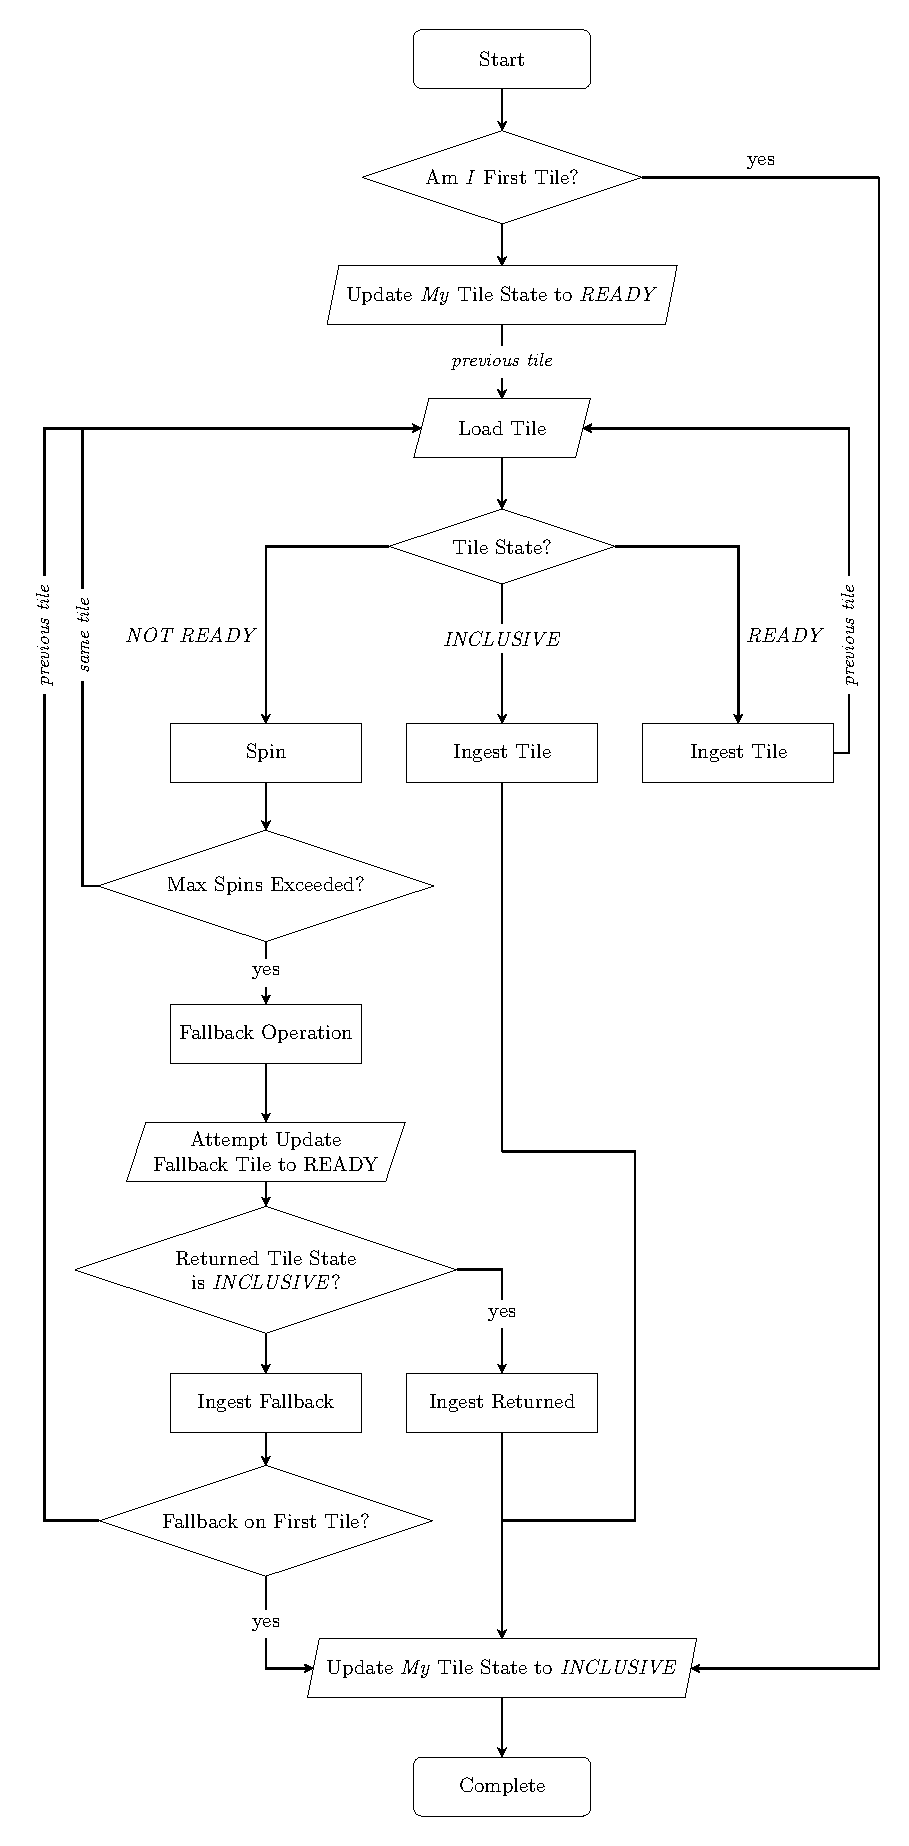
\includegraphics[width=\linewidth]{graphics/FlowChart.pdf}
  \label{fig:decoupled_fallback}
  \caption{Flow Chart Representation of Decoupled Fallback}
\end{figure}
\begin{enumerate}
  \item[(0)] \textbf{Posting Local Reduction:}
        \begin{itemize}
          \item Each workgroup posts its local reduction---the result of the workgroup-wide scan over partials---to global memory and updates its tile state to \emph{Ready}.
          \item If it is the first work tile, its local reduction \emph{is} its inclusive reduction. In this case, the workgroup updates its tile state directly to \emph{Inclusive} and bypasses the \emph{Chained-Propagation} phase entirely.
        \end{itemize}

  \item \textbf{Initialization:}
        \begin{itemize}
          \item The control flag, initialized to \emph{Locked}, signals that the workgroup should enter the \emph{Chained-Propagation} phase.
          \item The first thread initializes a \emph{previous reduction} variable in registers with $\epsilon$ to hold the accumulated reductions of preceding tiles.
          \item The first thread initializes a \emph{current tile} pointer to its immediate predecessor, with which it begins to traverse backwards through the spine.
        \end{itemize}

  \item \textbf{Lookback:}
        \begin{itemize}
          \item The first thread queries the state of \emph{current tile}.
                \begin{itemize}
                  \item If the tile is in the \emph{Ready} state, the workgroup ingests the value and sets \emph{current tile} to the preceding tile, repeating this step until reaching a tile that is \emph{Not Ready}.
                  \item If the tile is in the \emph{Inclusive} state, the workgroup ingests the value and proceeds directly to step~4.
                  \item If the tile is in the \emph{Not Ready} state, the first thread spins for a limited number of iterations, defined by the \emph{Maximum Spin Count}.
                        \begin{itemize}
                            \item If this count is exceeded, it exits the lookback loop and proceeds to step~3, leaving the control flag \emph{Locked} to signal to the workgroup that a fallback is required. Additionally, it copies \emph{current tile} into shared memory to broadcast the fallback tile identity to the workgroup.
                            \item Otherwise, it continues spinning until the tile transitions to a \emph{Ready} or \emph{Inclusive} state. Without FPG, \emph{Decoupled Lookback} risks spinning indefinitely and deadlocking at this stage.
                        \end{itemize}
                \end{itemize}
        \end{itemize}

  \item \textbf{Fallback:}
        \begin{itemize}
          \item If the blocking tile is still \emph{Not Ready} after waiting, the workgroup initiates a fallback operation.
          \item Using the tile index provided by the first thread, the full workgroup computes the reduction of the blocking tile by directly processing the corresponding elements. This process involves a \emph{workgroup-wide reduction},\footnote{See footnote NUMBER.} utilizing additional shared memory to aggregate partial subgroup results.
          \item Once the fallback reduction is complete, the workgroup \emph{attempts} to post the reduction to global memory and update the tile's state to \emph{Ready}.
          \item As this update attempt is performed atomically, the workgroup simultaneously reads back the blocking tile's most recent state:
                \begin{itemize}
                  \item If that most recent state is \emph{Inclusive}, the fallback value computed by the workgroup is discarded, and the first thread ingests the returned value before proceeding to step 4.
                  \item Otherwise, the first thread ingests the fallback value.
                        \begin{itemize}
                            \item If the blocking tile is the first in the spine, the workgroup has reached the start of the spine and has thus completed the lookback. The first thread proceeds to step 4.
                            \item Otherwise, the first thread updates \emph{current tile} to the preceding tile, returning to the lookback process in step~2.
                        \end{itemize}
                \end{itemize}
        \end{itemize}

  \item \textbf{Finalization:}
        \begin{itemize}
          \item To prioritize inter-workgroup reduction propagation, the first thread immediately adds the local reduction to \emph{previous reduction}, posts the inclusive reduction to global memory, and transitions the tile state to \emph{Inclusive}.
          \item It then writes \emph{previous reduction} to shared memory, allowing all threads to apply it in their \emph{workgroup-wide} and local scan computations.
          \item Finally, the first thread sets the control flag to \emph{Unlocked}, signaling the rest of the workgroup that \emph{Chained Propagation} has completed, and allowing the final write phase to begin.
        \end{itemize}
\end{enumerate}

\john{In this item + the previous item, I bet there's some ordering constraints, either for correctness or for performance. For instance, I bet the highest priority is to add the previous reduction to my reduction and posting the result, since that propagation speed across tiles is probably really important for performance. Perhaps worth pointing out. Does the flag-unset have any ordering constraints in terms of correctness?}
\thomas{Last phase may still need revision in accordance with above feedback. . . I have deliberately tried to avoid mentioning barriers to keep the section succinct.}
\john{I agree with your succinct strategy. I like that you now say reduction-propagation is the first priority, and why.}

\subsection{Tile State Implementation}
Since workgroups must observe updates from one another, but WebGPU lacks a \emph{volatile}-like qualifier, we rely on atomics to ensure visibility and consistency across workgroups. Because a tile may be in three possible states, two bits are required to record its state alongside the bits needed to store the tile's reduction value. Previous \emph{Chained-Scan} architectures relied on 64-bit atomics and/or memory fences to ensure a consistency between state and value, but WebGPU’s lack of a memory model \john{I'm not sure I would say ``lack of a memory model''. It's not the (lack of) memory model that's the problem. It's specifically that we don't have the operations that give us the behavior that we require. If we had the right operations that did the right thing but didn't have a memory model, we'd be fine. We want to specifically call out what is missing and what that means, and do so as generically as possible (not ``we are missing this specific atomic call'' but instead ``we are missing some sort of atomic call that has the following behavior''). Above, we want to not only say that we don't have a volatile qualifier but also both what that means and why it would be specifically useful if we had it. Doing the latter two things gives valuable ammunition to WebGPU and GPU architects that want to improve the API and hardware.} and 64-bit atomic support makes both infeasible. Instead, we use two or four 32-bit values, splitting the reduction value into 16-bit segments while reserving the two most significant bits of each 32-bit value to encode the tile state. \john{I would try to add a sentence or two on why we can't do the obvious thing---having the state in one word and the reduction value in a different word---and why the split value avoids that problem. This is not obvious to the reader.}
\begin{figure}[h!]
  \centering
  \includegraphics[width=\linewidth]{graphics/split.pdf}
\end{figure}

To accommodate the split values during \emph{Chained Propagation}, we use two or four threads from the first subgroup, leveraging subgroup \emph{ballot} to verify state consistency, and subgroup \emph{shuffle} to join and split reductions. With one thread per 16 bits and a minimum subgroup size of four in WebGPU, this method supports both 32-bit and 64-bit values, enabling 64-bit scans without 64-bit atomics or fences.\footnote{Although native 64-bit values are not currently supported by the WebGPU specification, their future inclusion is anticipated.}

Fallbacks require a tile state representation and an atomic operation that can safely transition a tile to \emph{Ready} without overwriting a more advanced state. When an update attempt is made, a blocking tile may be in any of the three states due to either of two scenarios: (1) a false-positive fallback on a tile that transitions to \emph{Ready} or \emph{Inclusive} before fallback completion, or (2) another workgroup completing its fallback first, leaving the tile in \emph{Ready}. WebGPU does not guarantee the correctness of atomic \emph{Compare-and-Swap} across all devices, inhibiting its use. \john{Is CAS the traditional/common way to implement this? If so, say so, and if you can, provide a cite, even if it's not a formal cite but just the name of another package that uses this strategy.} Instead, we encode the tile state in the most significant bits of the split value and enforce a strict state ordering: \emph{Inclusive} $>$ \emph{Ready} $>$ \emph{Not Ready}. This allows an atomic \emph{maximum}, which successfully updates to a more advanced state but prevents a state regression, to correctly perform updates.

\section{Evaluation}
\subsection{Experimental Setup}
We configure workgroups with a size of 256 threads, where each thread processes 4 vectors of size 4, resulting in 16 elements per thread and a total work tile size of 4096. We find a maximum spin count of 4 as offering good responsiveness to blocking, while minimizing false-positives fallbacks. As the size of the local spine is inversely proportional to the subgroup size, we allocate sufficient shared memory to accommodate the minimum subgroup size specified by the WebGPU standard, which is 4. Despite the additional shared memory required for conflict avoidance and fallback operations, total shared memory usage remains modest at only 1 KB. For all tests, we use an input size of $2^{25}$.

Something about devices here.
\subsection{Performance Comparison}
To evaluate the performance of \emph{Decoupled-Fallback}, we compare it against two key benchmarks: \emph{Reduce-Then-Scan} (RTS) and a \emph{Memcopy} operation. RTS serves as a baseline to demonstrate the performance gains of our approach over the previous FPG-constrained technique. Memcopy is included as a point of reference, as it shares the same $2n$ global memory movement required by scan operations.

\thomas{Forgot about tables. Mega table incoming.}

\thomas{Performance is good}

\subsection{How (un)fair is fair?}
Show the stats of each device. How many lookbacks?  How many fallbacks initiated? How many successful fallbacks?

\subsection{Emulated Blocking}
To demonstrate the resilience of our technique under fallback rates significantly higher than those observed organically on devices, we intentionally force fallbacks by omitting the posting of work tile reductions. Starting with infrequent omissions---1 in 512 workgroups---we progressively increase the rate to near-continuous levels, reaching 1 in 2 workgroups.
\begin{figure}
  \centering
  \begin{subfigure}{.9\linewidth}
    \centering
    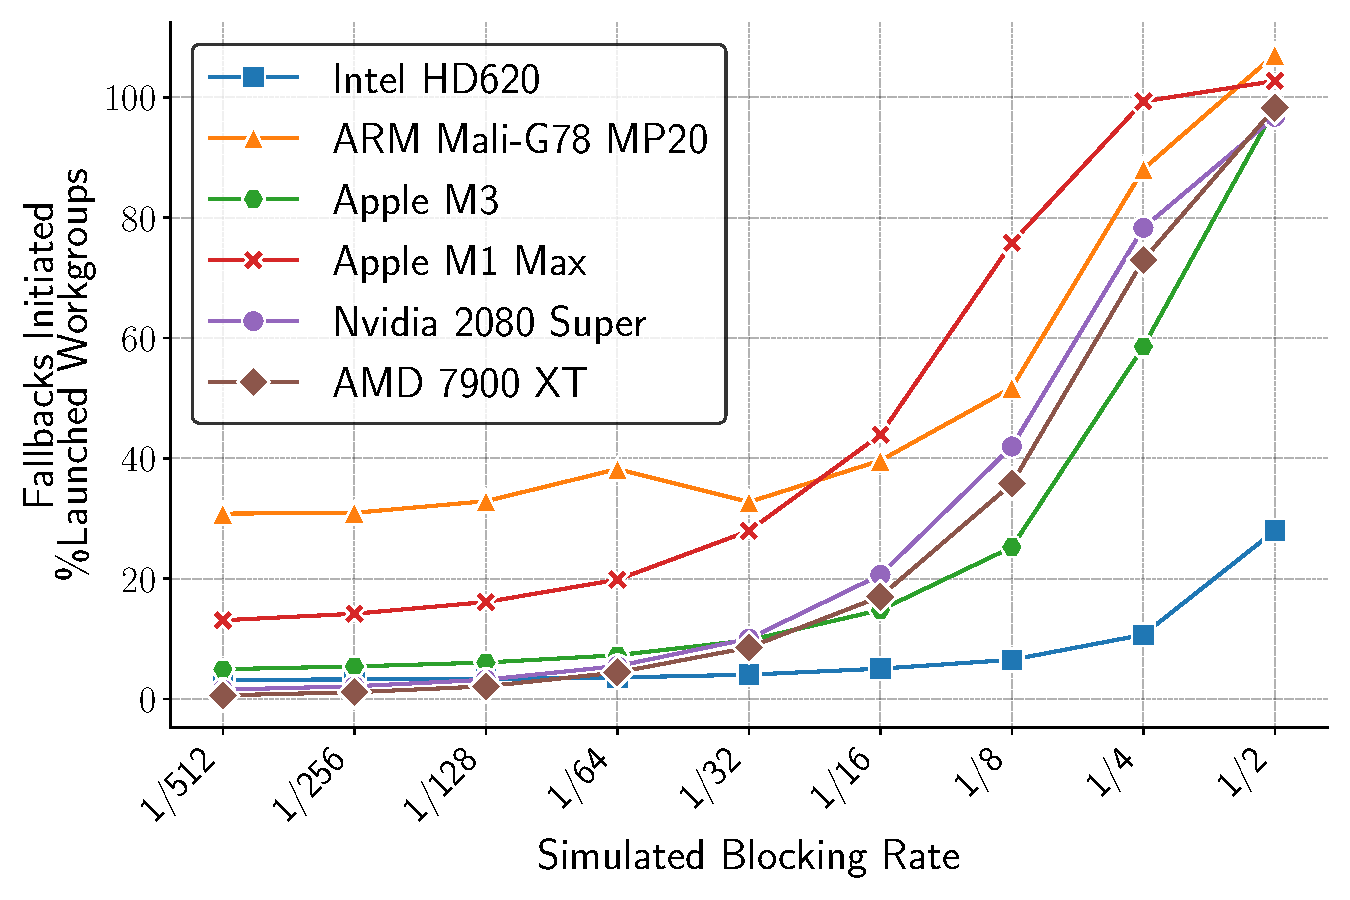
\includegraphics[width=\linewidth]{graphics/fallbacksInitiated_plot.pdf}
    \caption{Fallbacks Initiated}
    \label{fig:fallbacks_initiated}
  \end{subfigure}
  \begin{subfigure}{.9\linewidth}
    \centering
    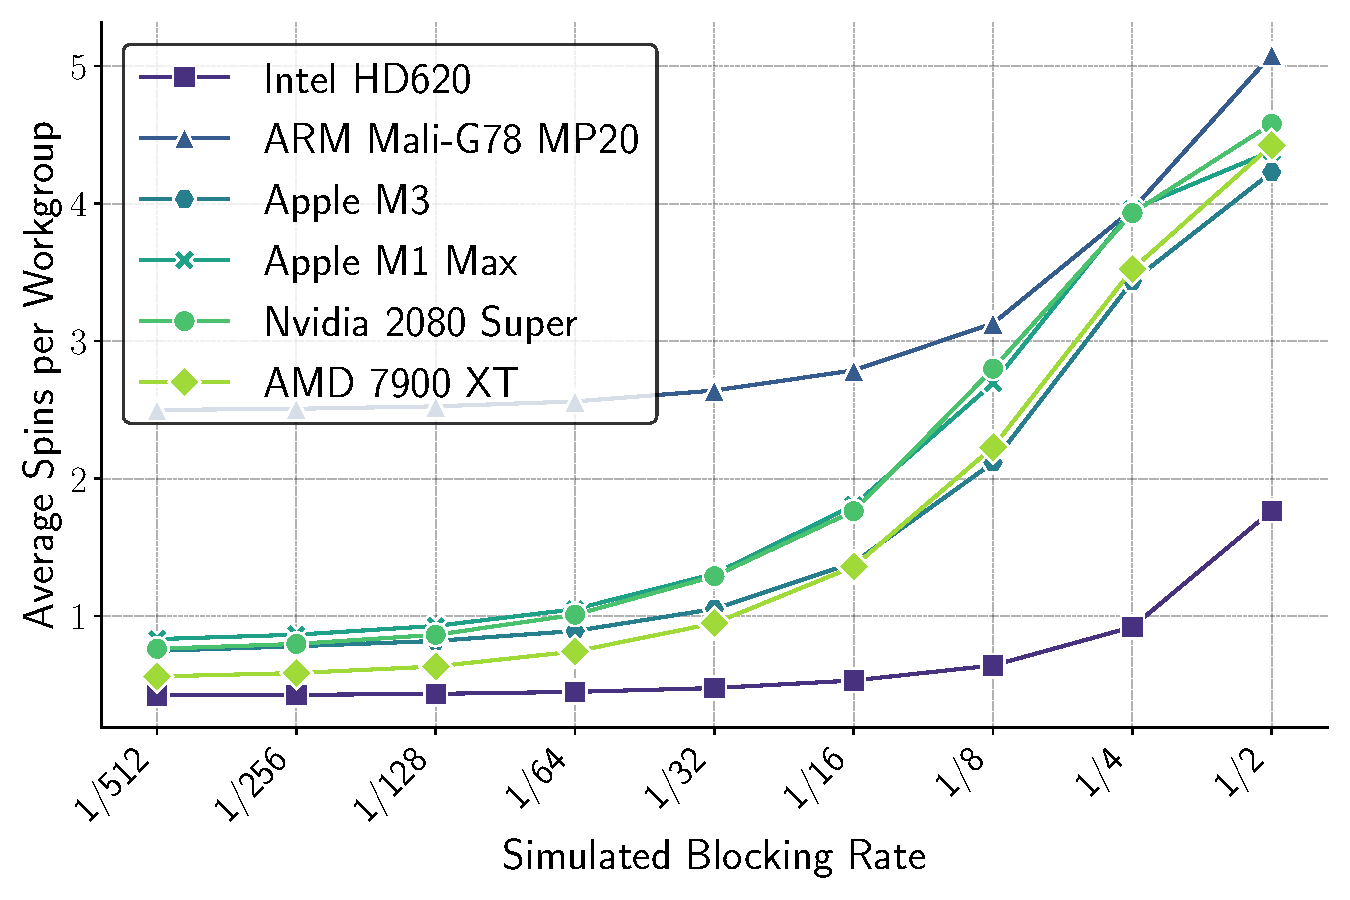
\includegraphics[width=\linewidth]{graphics/totalSpins_plot.pdf}
    \caption{Total Spins}
    \label{fig:total_spins}
  \end{subfigure}
  \begin{subfigure}{.9\linewidth}
    \centering
    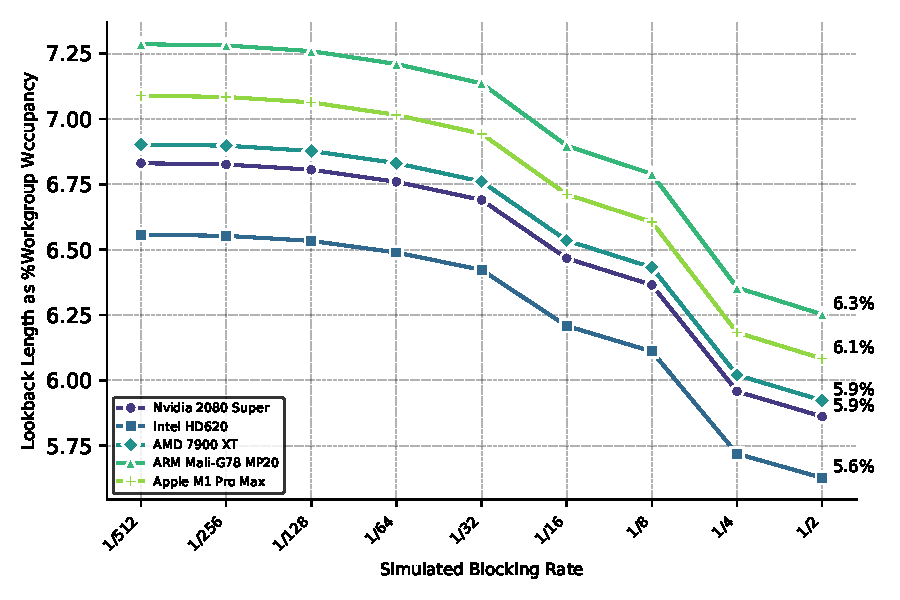
\includegraphics[width=\linewidth]{graphics/lookbackLength_plot.pdf}
    \caption{Lookback Length}
    \label{fig:lookback_length}
  \end{subfigure}
  \begin{subfigure}{.9\linewidth}
    \centering
    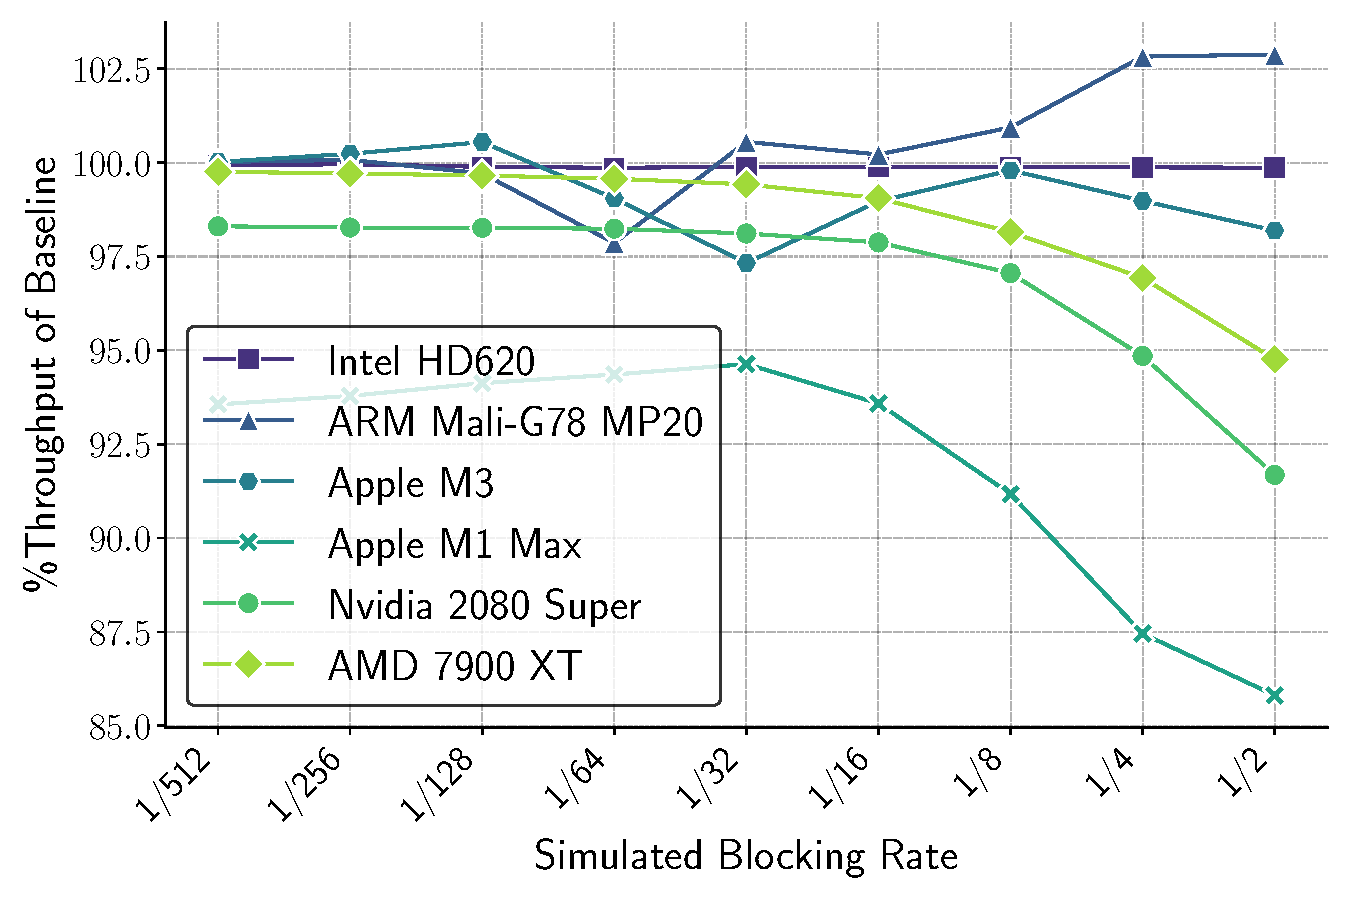
\includegraphics[width=\linewidth]{graphics/time_plot.pdf}
    \caption{Speed vs Memcopy}
    \label{fig:execution_time}
  \end{subfigure}
  \caption{Simulated Blocking\john{Text in these plots---axis labels, etc.---needs to be larger. If it's significantly smaller than body text, which it is, it's just not legible.}}
  \label{fig:vertical_images}
\end{figure}

In Figure~\ref{fig:fallbacks_initiated}, we measure the number of fallbacks proportional to the number of workgroups launched, and verify that we are indeed inducing fallbacks. In Figure~\ref{fig:total_spins} we measure \thomas{this should be spins per workgroup it's a better metric}. In Figure~\ref{fig:lookbackLength} we see that. Finally, in Figure~\ref{fig:execution_time}, we can see that, even when \emph{half} the workgroups are deadlocking, \emph{Decoupled-Fallback} still achieves speeds of . . .

\section{Discussion}

\subsection{Trade-offs}

\subsection{Limits on Speed-of-Light Performance}
There are a number of factors which may preclude speed-of-light performance, but most salient is the fairness of the scheduling model. In \emph{Decoupled-Fallback}, a work tile which is late due to unfairness is indistinguishable from one which is blocking, so as a scheduler becomes increasingly unfair, it incurs an increasing number of redundant fallbacks. Consider a hardware with a workgroup occupancy denoted by $o$, and let $f$ represent the probability that a fallback operation occurs at a particular lookback step. Because the number of lookback steps is bounded by $o$, the expected number of fallback operations is approximately $fo$. This results in a factor of $fo$ increase in global memory reads and a factor of $fo\log{n}$ increase in work.

This increased sensitivity to fairness exacerbates existing issues which negatively impact the performance of previous scan architectures, namely lack of compute, and slow atomic update latency. On hardware that lacks sufficient compute power to be memory-bandwidth bound, the additional work incurred by redundant fallback reductions is particularly deleterious. High atomic update latency further compounds the problem: as inter-workgroup communication time grows, the minimum delay before updates become visible to dependent workgroups also increases. This, in turn, raises the number of lookback steps that may be needed and potentially leads to redundant fallbacks.

\thomas{Somewhere in here is perfect for Raph's commentary on the speed of atomics on different hardware. Once we have it, we can retool this section around it.}

\begin{acks}
\end{acks}

\bibliographystyle{ACM-Reference-Format}
\bibliography{bib}

\clearpage
\appendix
\section{Artifact}

\subsection{Availability}
We provide our artifact in the following GitHub repository:
\thomas{Will anonymize with GithubAnonymous once we are ready.}.

\subsection{API Choice}
As rust is significantly more easy to build across devices we chose the WGPU api.

\subsection{Device Choices}
We chose a diverse range of devices to illustrate

\subsection{Baseline Comparisons}
Since WebGPU limits device-side timestamps to compute or render passes, we implement a custom Memcopy kernel for timing purposes. Similarly, as there are no existing WebGPU implementations of RTS, we rely on our own optimized version for comparison. To ensure a competitive evaluation, our RTS implementation employs a variable-launch main kernel with a single workgroup performing a serial spine scan, as we found raking to be less performant in practice. Apart from this adjustment, the intraworkgroup implementation in RTS is identical to that used in \emph{Decoupled-Fallback}.

\end{document}
\endinput

%%% Local Variables:
%%% mode: LaTeX
%%% TeX-master: t
%%% End:
